% Section content template for individual Educative lessons
% This file contains the actual content for a specific section
% Generated from Educative API section content

% Section: Abstraction
% Section ID: 4989957095817216
% Section Slug: abstraction
% Generated: 2025-12-16T12:48:46.706434

\subsection{Definition}\label{ybycftmSRof_QkXnEZA3H-1}
\\
\textbf{Abstraction} is a technique used in object-oriented programming that simplifies the program\textquotesingle s structure. It focuses only on revealing the necessary details of a system and hiding irrelevant information to minimize its complexity. In simpler words, we can say that it means to show what an object does and hides how it does it.

\subsection{Example}\label{FiI9quxOmwL-h0dS9Lmbm}
\\
There are countless real-life examples demonstrating the principle of abstraction. Consider the ``volume'' button on a television remote. With one click, we can increase the TV's volume. Internally , this button might call a function like \texttt{volumeUp()}. The TV then responds by producing louder sound. As users, we don\textquotesingle t need to know anything about the internal circuitry or mechanism. We simply know that pressing the button increases the volume.
\\
Another example is our everyday use of vehicles. Pressing the accelerator pedal signals the car to increase its speed by consuming more fuel. We don\textquotesingle t need to understand the detailed mechanical processes involved; we only interact with the simplified interface provided to us.

\begin{figure}[htbp]
 \centering
 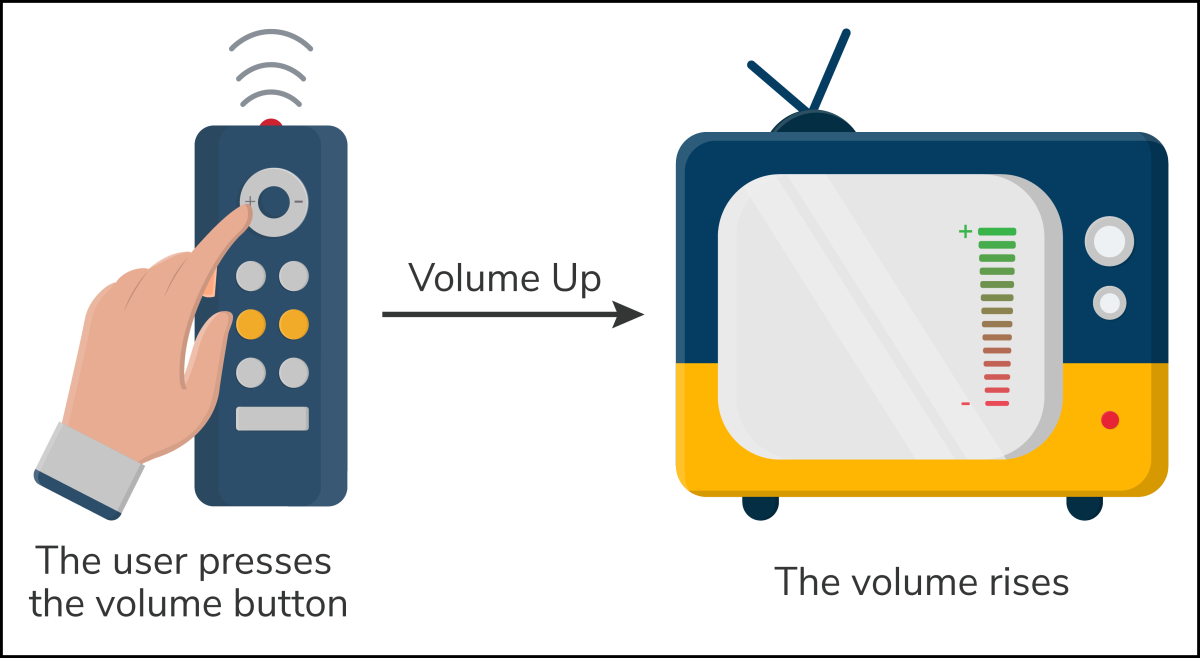
\includegraphics[width=0.5\textwidth]{Images/chapter_2/section_4989957095817216/5436658545852416.png}
 \caption{Abstraction in the form of the "volume up" button}
\end{figure}

\subsection{Implementation of abstraction in programming languages}\label{ybycftmSRof_QkXnEZA3H-2}
\\
So, let's put all this theory into practice. In the code below, we have a basic class of a circle:

\textbf{Attributes of the Circle class}

\begin{lstlisting}[language=Java]
class Circle {
  private double radius;
  private double pi;
};
\end{lstlisting}

It has two variables, \texttt{radius} and \texttt{pi}. Now let's add the constructor and functions to calculate the area and perimeter:

\textbf{Abstraction implementation in programming languages}

\begin{lstlisting}[language=Java]
class Circle {

  //define data attributes

  private double radius;

  private double pi;

  

  //define constructors

  public Circle() {

    radius = 0;

    pi = 3.142;

  }



  public Circle(double r) {

    radius = r;

    pi = 3.142;

  }

  

  //define methods

  public double area() {

    return pi * radius * radius;

  }



  public double perimeter() {

    return 2 * pi * radius;

  }  

  

  public static void main(String[] args) {

    Circle circle = new Circle(5);

    System.out.printf("Area: %.2f %n", circle.area());

    System.out.printf("Perimeter: %.2f %n", circle.perimeter());

  }

}
\end{lstlisting}

As you can see, we only need to define the radius of the circle in the constructor. After that, the \texttt{area()} and \texttt{perimeter()} functions are available to us. This interface is part of encapsulation.
\\
We use the functions to calculate the area and perimeter. Users do not need to know the implementation details of the functions. Even \texttt{pi} is hidden since it's a constant. This is how we can achieve abstraction using classes.

\subsection{Advantages of abstraction}\label{XCJW7e-AXwdYx2ZHlSxfb}
\\
The following are some advantages of abstraction:

\begin{itemize}
\item
\protect\phantomsection\label{GQoChZIDe6_ko65YMF-l9}
It reduces the complexity of the system from a user\textquotesingle s perspective.
\item
\protect\phantomsection\label{gc4G9GW2tFLv2BPoPOivA}
It makes the code extendable and reusable.
\item
\protect\phantomsection\label{DIloc5HQeKaMfRqKko_EP}
It refines the modularity of the application or the system.
\item
\protect\phantomsection\label{IBfw-s4WoTrgsR5S8Smf7}
It makes the code more maintainable.
\end{itemize}

\subsection{Abstraction vs. encapsulation}\label{2WiTRiThVea4dNqTw2fgZ}
\\
Since abstraction and encapsulation are data hiding techniques of OOP, they are often confused with being the same. Let
\textquotesingle s look at some of the differences in the following table:

\begin{table}[htbp]
\centering
\small
\adjustbox{max width=\textwidth}{
\begin{tabular}{|p{0.482\textwidth}|p{0.468\textwidth}|}
\hline
\textbf{Abstraction} & \textbf{Encapsulation} \\
\hline
\hline
It focuses on the design level of the system. & It focuses on the application level of the system. \\
\hline
It hides unnecessary data to simplify the structure. & It restricts access to data to prevent its misuse. \\
\hline
It highlights the work that the object performs. & It deals with the internal working of the object. \\
\hline
Abstraction means to hide implementation using interface and abstract classes. & Encapsulation means to hide data using getter and setter functions. \\
\hline
\end{tabular}
}
\end{table}

Next, let\textquotesingle s look at another important principle of object-oriented programming---inheritance.

% End of section content